
\begin{figure}[hbt]
	\centering
  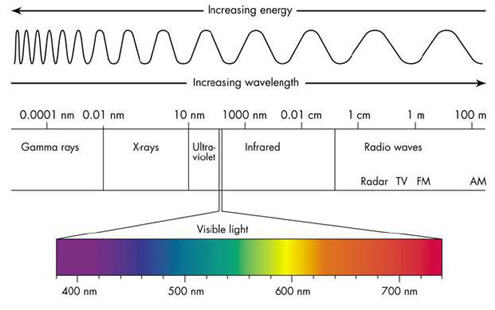
\includegraphics[height=200px]{img/wavelengths}
  \caption{Wavelengths, visible light band}
  \label{fig:wavelength}
\end{figure}

%intro
Visible Light Communication is a form of optical communication that uses signals in the visible light band to transmit information.
Contrary to the more common fiber-optic communication, VLC is wireless, and transmitted over free space.
Typically, normal fluorescent lamps or LEDs, rather than complex communication devices,  are used to transmit in VLC.
In general, receivers are electronic devices that include one or more photoresistors, in order to measure light signals from a source.
In some cases, digital cameras can also be used to form a receiver. \todo{cite use of digital camera}
%http://visiblelightcomm.com/

% from Wikipedia : VLC can be used as a communications medium for ubiquitous computing, because light-producing devices (such as indoor/outdoor lamps, TVs, traffic signs, commercial displays and car headlights/taillights[4]) are used everywhere.[3] Using visible light is also less dangerous for high-power applications because humans can perceive it and act to protect their eyes from damage.

%optical
\subsection{Optical Communication}
[photophone, optical fiber, infrared, ultraviolet]

Optical communication is allegedly one of the oldest types of communication from a distance in the history of human kind.
Examples of early communication techniques that use light to carry signals can be traced back millennia, with the first lighthouses, navigation lights, beacon fires that would assist in navigation or communicate danger.
It is only with the spread of electricity though, that optical communication technologies could really develop.
Many trace the start of Visible Light Technology to 1880, when Alexander Graham Bell and Charles Sumner Tainter invented the photophone, a device able to transmit wireless voice messages over several hundred meters modulating sunlight. \todo{reference to photophone}
Since then, optical communication has been developed to include many different variants, the most common  of which is \textbf{fiber optic communication}. \todo{talk fiber}
Other common optical communication technologies include \textbf{infrared} light (IR) and \textbf{ultraviolet} (UV). \todo{talk IR and UV}

%ronja
\subsection{RONJA}
%http://ronja.twibright.com/
\todo{talk RONJA}

%lifi
\subsection{Li-Fi}
The term Li-Fi was first introduced by a german physicist, Harald Haas, co-founder of PureLiFi, in occasion of a TED Global talk on Visible Light Communication in 2011. \cite{tedtalk}
Since then, the term has been reported in many articles and has gained popularity as a common synonymous for Visible Light Communication.
After the name was adopted by the Optical Wireless Communication (OWC) community with the launch of the LiFi Consortium in 2011, an industry group that promotes OWC technologies, it can be sometimes extended to describe general wireless data access points that use light, visible or otherwise.
This includes also the infra-red and ultraviolet band.\\

The main reason why this technology is quickly gaining popularity in the research is because it potentially allows to unlock a vast amount of electromagnetic spectrum in the visible light region, unused for transmission.\cite{haas1}
This has been seen as a promising reaction to the saturation of the Radio Frequency (RF) spectrum, a very likely outcome of the huge success of wireless technology, also predicted by the US Federal Communication Commission\cite{crisis}. 

A second reason is that transmission through light can achieve surprising high speeds.
Starting from 2010, research had been able to improve the transmission rate further and further.
In his TED talk in 2011 Haas demonstrated real time video streaming from a white LED at data rates up to 130 Mbps\cite{tedtalk}, while another group achieved over 513 Mbps\cite{500Mbps}.
In the following years, there have been continuous reports of improved data rates in transmission.
A single white LED has been proven to transmit from about 1 Gbps\cite{1Gbps}, up to 3.5 Gbps\cite{3.5Gbps}, while 3.4 Gbps have been demonstrated with a single RGB LED\cite{3.4Gbps}.\\
This rates can be further improved by the use of arrays of light sources and more complex systems.
The Mexican software company Sisoft together with scientists from the Autonomous Technological
Institute of Mexico in 2014 reached the surprising data rate of 10 Gbps, setting the record.\\
Other appealing aspects to this technology are the low cost of implementation for the use of off-the-shelf LED bulbs and its security, for the reason that communication can be eavesdropped only in direct line of sight within short distance.\\
 
There are a few groups that are leading the research in the field of Visible Light Communication.
One of these is the Li-Fi R\&D Centre at the University of Edinburgh, of which prof. Harald Haas is the director.
Another very important research group operating in the same area is Disney Research, often in collaboration with ETH Zurich.
Another group worth mentioning is the Li-Fi Consortium, an international organisation formed by companies in optical wireless communication technology and research institutes.
A good part of the research is also carried out by multiple other research groups worldwide, especially in Asia and India in particular.

\todo{expand, and also add some applied robotics arguments, and communication}

%standards
\subsection{Standard and specifications}
\label{modulschemes}
Visible light communication is regulated by a standard similar to the one of wireless networks, in the same IEEE 802 family.\cite{IEEE}
The IEEE 802.15.7 standard defines a draft of the physical layer (PHY) and the media access control (MAC) layer for VLC. 
According to Gordon Povey, former CEO at PureLiFi\cite{poveyspec}, the MAC layer as of April 2011 supports three multiple access topologies: peer-to-peer, star configuration and broadcast mode.\\
The Physical layer is divided into three types, that use different modulation schemes.
The three modulation schemes are: 
\begin{itemize}
\item On-Off Keying
\item Variable pulse position modulation (VPPM)
\item Colour shift keying (CSK)
\end{itemize}
\textbf{On-Off Keying}\newline
On-Off Keying is the simplest modulation scheme. 
In this scheme, a digital 1 is represented by the light state being on, and 0 otherwise.
In the 802.15.7 standard, Manchester coding is used to ensure the period of each pulse is the same.
This type of encoding, instead of having a digital 0 represented by a low signal and a digital 1 by a high signal, encodes each data bit as either low then high (1), or high then low (0), in equal time.\\
\newline
\begin{figure}[H]
\centering
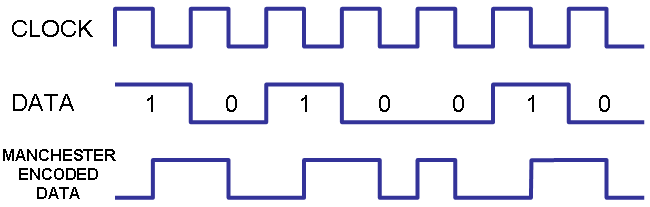
\includegraphics[scale=0.3]{img/ookmodulation}
\caption{OOK modulation using Manchester coding.}
\label{fig:ookmod}
\end{figure}
\textbf{Variable pulse position modulation (VPPM)}\newline
VPPM is similar to pulse position modulation (PPM), in which the data is encoded using the position of the pulse within a set time period.
In this modulation scheme, light dimming is allowed as long as the period containing the pulse is long enough to allow different positions to be identified. 
As in the Manchester coding a positive pulse at the beginning of the period followed by a negative pulse at the end can represent a digital 0, and a 1 is represented by a negative pulse at the beginning followed by a positive one at the end.\\
\newline
\begin{figure}[H]
\centering
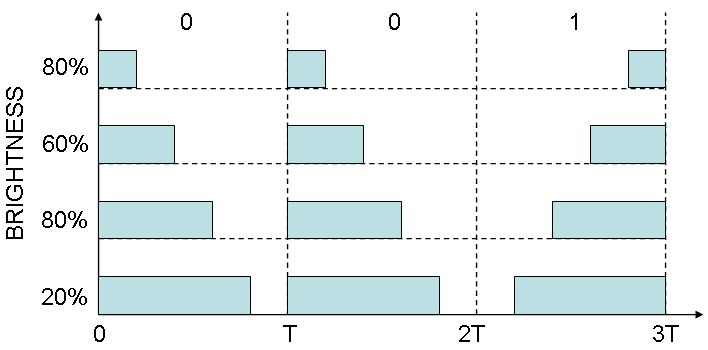
\includegraphics[scale=0.3]{img/VPPM}
\caption{Variable pulse position modulation to support light dimming.}
\label{fig:ookmod}
\end{figure}
\textbf{Colour shift keying (CSK)}\newline
This scheme allows the light intensity to be constant by encoding the information in the colour of the light.
For implementing this kind of transmission the system must use RGB type LEDs.

%other technologies
\subsection{Comparison with other technologies}
compare ranges and speeds, maybe also bands